\begin{figure}[htbp]
    \centering{}
    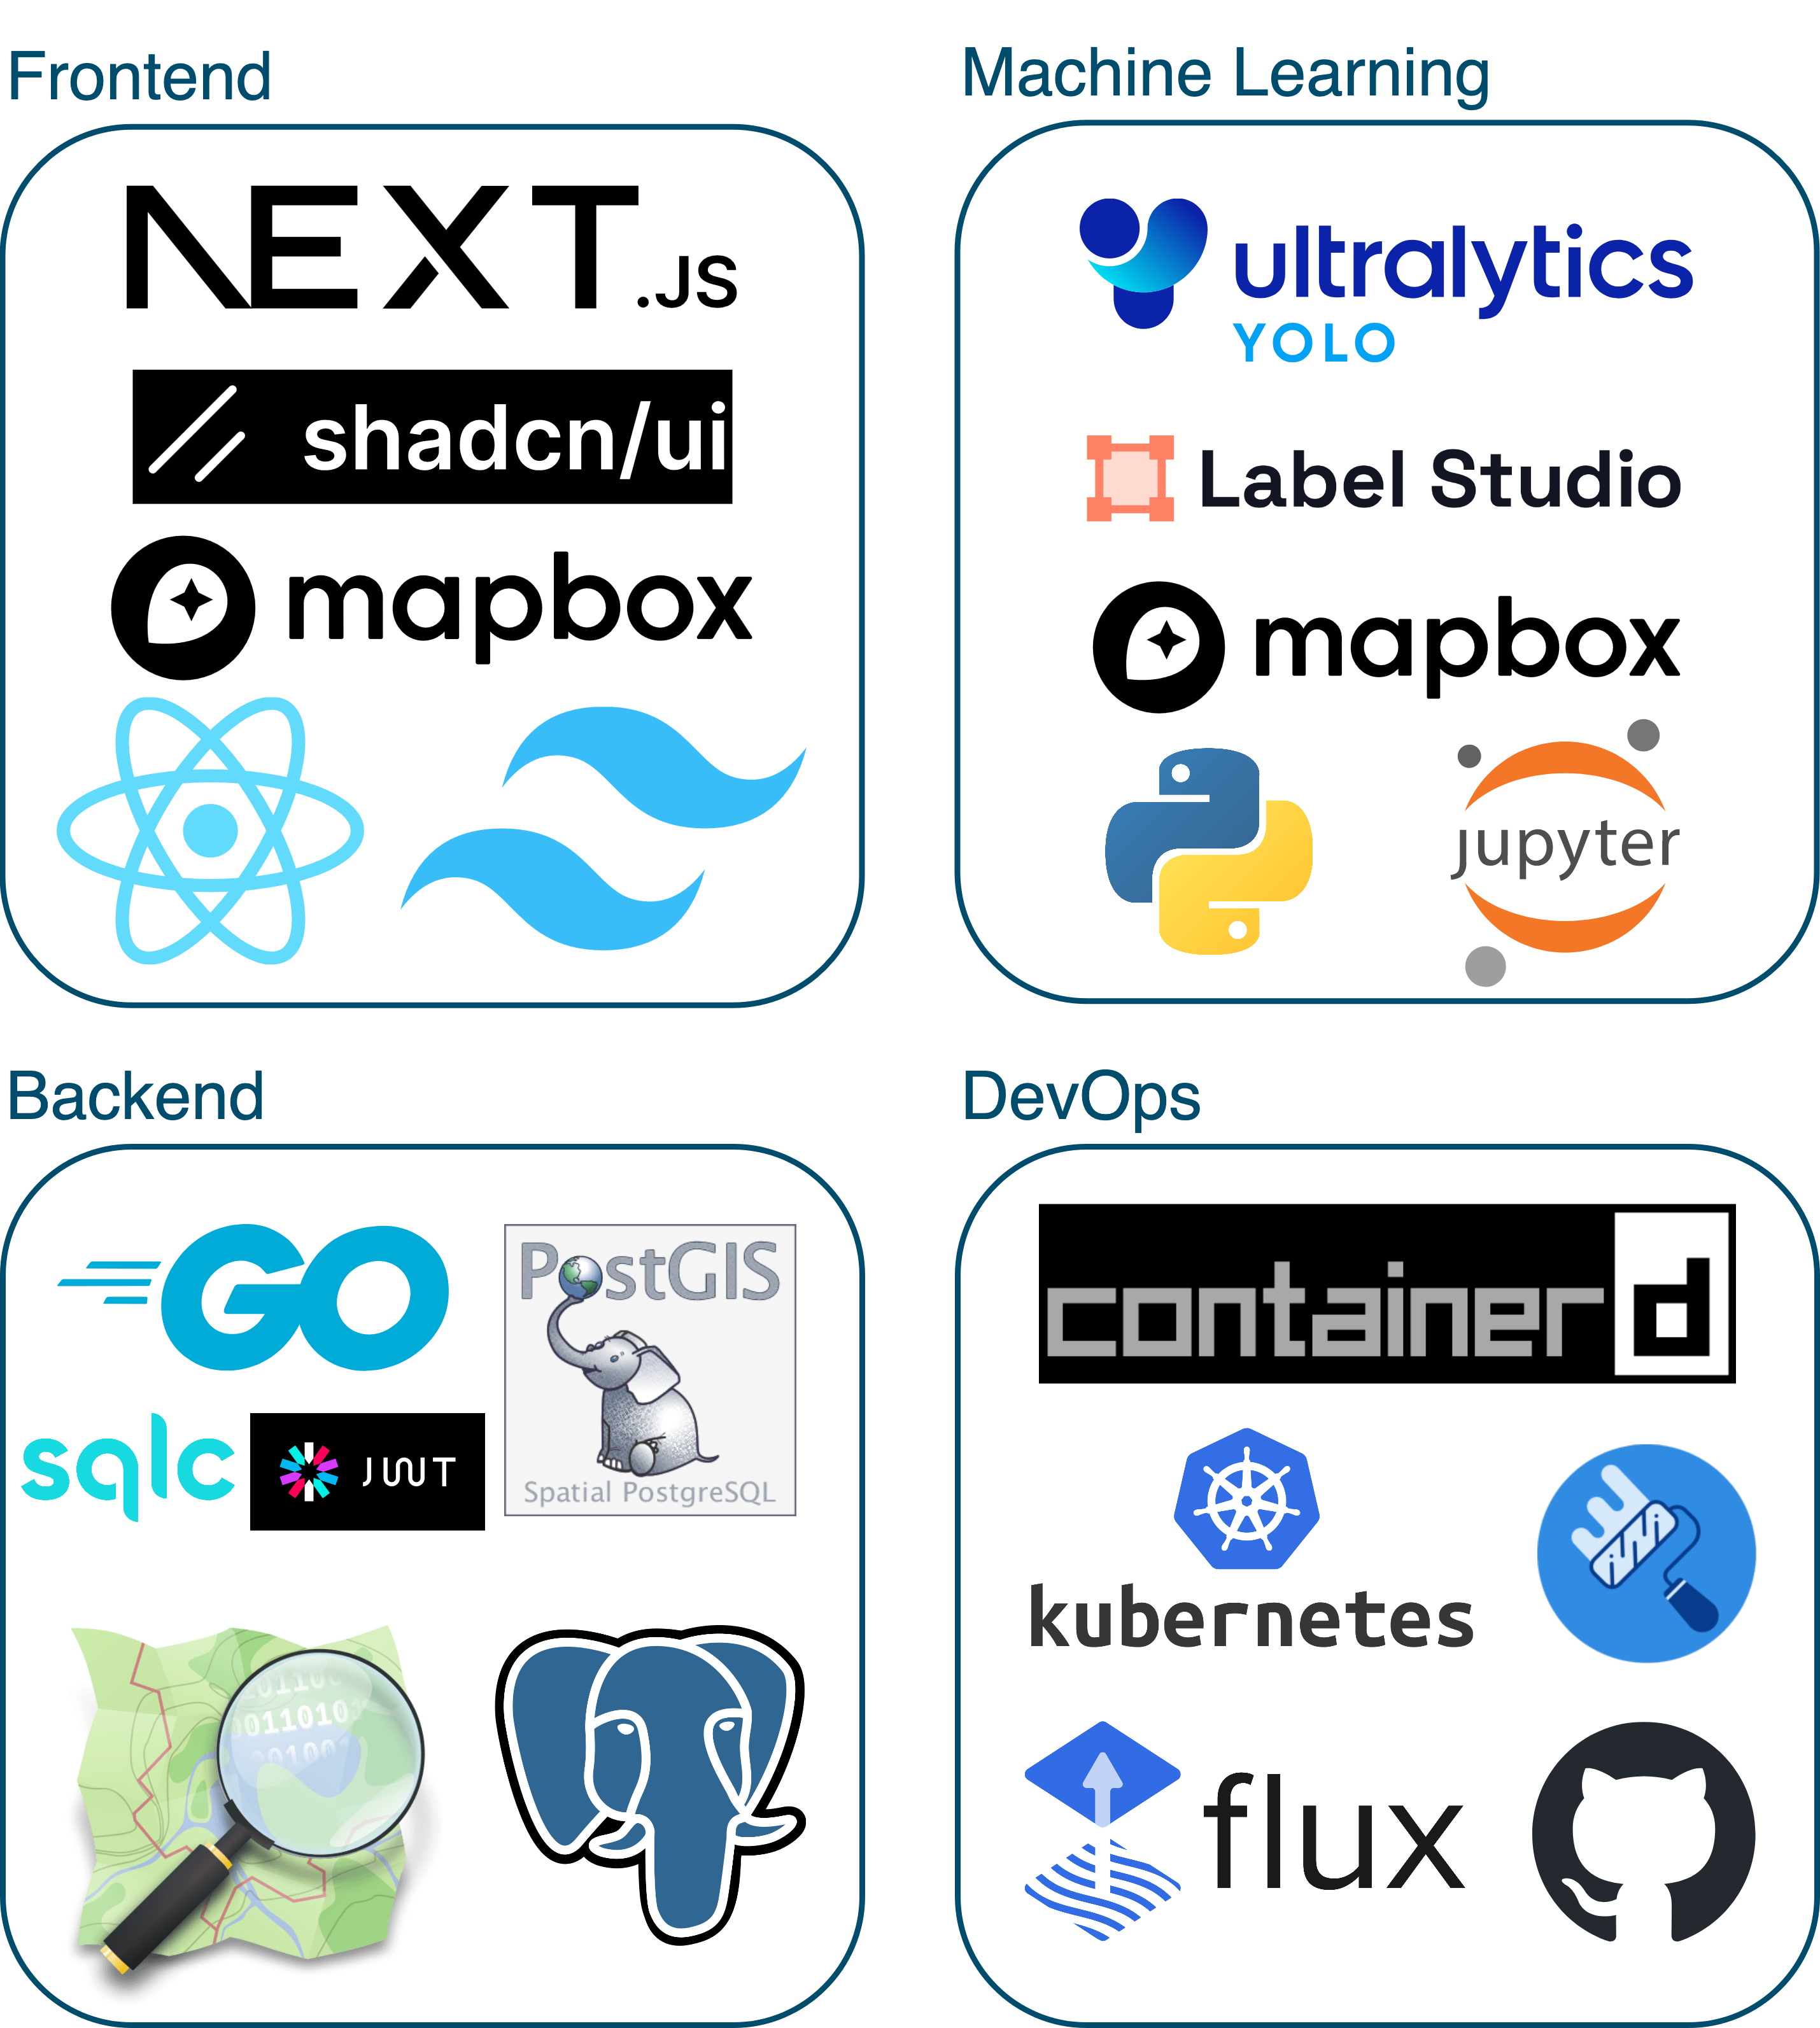
\includegraphics[width=0.5\textwidth]{images/stack_grid.png}
    \caption{Magpie's technology Stack}
\end{figure}

\subsubsection{Frontend Technologies}

The frontend stack plays a critical role in providing a smooth and interactive user experience for the application. It is built on top of modern web technologies, each serving a unique purpose:

\begin{itemize}
    \item{} \textbf{Next.js:} This React framework offers server{-}side rendering (SSR) and static site generation (SSG), which improve performance, SEO, and user experience.
    \item{} \textbf{React:} As the foundation of the frontend, React allows for component{-}based development, making the interface scalable and easy to maintain.
    \item{} \textbf{TailwindCSS:} A utility{-}first CSS framework that simplifies styling by providing ready{-}to{-}use classes, enabling rapid UI development.
    \item{} \textbf{shadcn/ui:} A collection of reusable UI components that work seamlessly with Next.js and React, enhancing productivity and consistency across the application.
    \item{} \textbf{Mapbox:} A powerful mapping platform that enables interactive, customizable maps. It helps visualize geospatial data effectively, which is key for location{-}based services in this project.
\end{itemize}

These technologies combine to create an engaging user interface that is both functional and visually appealing, allowing users to interact with location{-}based data and services efficiently.

\subsubsection{Machine Learning Technologies}

The machine learning stack adds intelligent capabilities to the system, enabling advanced features such as object detection. Here’s a breakdown of the tools in this section: 

\begin{itemize}
    \item{} \textbf{Ultralytics YOLO:}  An object detection model that helps identify specific objects in images, enhancing the system's ability to recognize and interpret visual data. 
    \item{} \textbf{Label Studio:} A flexible tool for annotating datasets, enabling easy labeling of images, text, and audio. This is crucial for creating high-quality datasets to train machine learning models like YOLO. 
    \item{} \textbf{Python:} The primary language for developing our scripts and running machine learning models, Python supports image processing, model training, and analysis. 
    \item{} \textbf{Jupyter Notebooks:} An interactive platform that allows data scientists to experiment with code, visualize results, and document their machine learning processes. 
\end{itemize}

These technologies allow the application to process and analyse data intelligently, enabling features such as object recognition in geographical data and personalized insights.

\subsubsection{Backend Technologies}

The backend stack ensures the application can handle large volumes of data, manage user requests, and perform complex computations. Some of the key technologies include:

\begin{itemize}
    \item{} \textbf{Go (Golang):} A highly performant programming language ideal for building scalable backend services.
    \item{} \textbf{PostGIS:}  An extension of \textbf{PostgreSQL}, PostGIS adds geographic object support to the database, making it easier to work with spatial data like maps, coordinates, and distance calculations.
    \item{} \textbf{sqlc:} A SQL code generator that helps developers write type{-}safe database queries in Go, reducing the chances of errors during database interactions.
    \item{} \textbf{JWT:} A compact, URL{-}safe token format used for securely transmitting information between parties, often for authentication and authorization purposes.
\end{itemize}

By leveraging these tools, the backend is capable of managing complex spatial data, performing queries on geospatial data, and ensuring smooth user interactions through highly responsive APIs.

\subsubsection{DevOps Technologies}

The DevOps stack ensures that the infrastructure supporting the application is reliable, scalable, and easily deployable. Key technologies in this section include:

\begin{itemize}
    \item{}  \textbf{Containerd:} A core container runtime that manages containerized applications, ensuring consistency across different environments (development, staging, production).
    \item{} \textbf{Kubernetes:} An orchestration platform for automating the deployment, scaling, and management of containerized applications. It allows the system to scale effortlessly based on demand and ensures high availability.
    \item{} \textbf{Flux:} A tool for continuous delivery and GitOps, Flux automates deployments by integrating with Git repositories. Changes made to the codebase are automatically reflected in the deployed infrastructure, ensuring consistency and reducing manual intervention.
    \item{} \textbf{GitHub:} The widely{-}used platform for version control and collaboration. GitHub supports seamless development workflows by enabling pull requests, code reviews, and version tracking.
\end{itemize}

Together, these tools create a robust DevOps pipeline that automates deployment, enhances reliability, and ensures that the application can handle scaling demands as it grows.

\subsubsection{Integration and Synergy}

The combination of frontend, backend, machine learning, and DevOps technologies ensures that the system functions as a seamless whole. Here's how the different parts work together:

\begin{itemize}
    \item{} The \textbf{frontend} presents an intuitive interface to users, allowing them to interact with location data, maps, and insights.
    \item{} The \textbf{backend} handles the heavy lifting, managing the spatial data, processing queries, and supporting dynamic content through APIs.
    \item{} \textbf{Machine learning} capabilities add intelligence to the system, enabling features like real{-}time object detection and personalized data analysis.
    \item{} \textbf{DevOps} practices ensure that the entire application can be deployed and scaled efficiently, with smooth continuous integration and deployment pipelines.
\end{itemize}

In conclusion, this tech stack forms a cohesive, scalable, and intelligent system. From object detection and efficient spatial data management to automated deployment pipelines, the technologies complement each other, resulting in a high{-}performance, feature{-}rich application.